\hypertarget{occt__tutorial_sec1}{}\section{Overview}\label{occt__tutorial_sec1}
This tutorial will teach you how to use Open C\+A\+S\+C\+A\+DE Technology services to model a 3D object. The purpose of this tutorial is not to describe all Open C\+A\+S\+C\+A\+DE Technology classes but to help you start thinking in terms of Open C\+A\+S\+C\+A\+DE Technology as a tool.\hypertarget{occt__tutorial_OCCT_TUTORIAL_SUB1_1}{}\subsection{Prerequisites}\label{occt__tutorial_OCCT_TUTORIAL_SUB1_1}
This tutorial assumes that you have experience in using and setting up C++. From a programming standpoint, Open C\+A\+S\+C\+A\+DE Technology is designed to enhance your C++ tools with 3D modeling classes, methods and functions. The combination of all these resources will allow you to create substantial applications.\hypertarget{occt__tutorial_OCCT_TUTORIAL_SUB1_2}{}\subsection{The Model}\label{occt__tutorial_OCCT_TUTORIAL_SUB1_2}
To illustrate the use of classes provided in the 3D geometric modeling toolkits, you will create a bottle as shown\+:


\begin{DoxyImageNoCaption}
\begin{center}
   \mbox{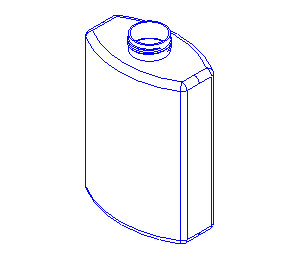
\includegraphics[width=240]{tutorial_image001.png}}
\end{center}
\end{DoxyImageNoCaption}


In the tutorial we will create, step-\/by-\/step, a function that will model a bottle as shown above. You will find the complete source code of this tutorial, including the very function {\itshape Make\+Bottle} in the distribution of Open C\+A\+S\+C\+A\+DE Technology. The function body is provided in the file samples/qt/\+Tutorial/src/\+Make\+Bottle.\+cxx.\hypertarget{occt__tutorial_OCCT_TUTORIAL_SUB1_3}{}\subsection{Model Specifications}\label{occt__tutorial_OCCT_TUTORIAL_SUB1_3}
We first define the bottle specifications as follows\+:

\tabulinesep=1mm
\begin{longtabu} spread 0pt [c]{*{3}{|X[-1]}|}
\hline
\rowcolor{\tableheadbgcolor}\PBS\centering \textbf{ Object Parameter }&\PBS\centering \textbf{ Parameter Name }&\PBS\centering \textbf{ Parameter Value  }\\\cline{1-3}
\endfirsthead
\hline
\endfoot
\hline
\rowcolor{\tableheadbgcolor}\PBS\centering \textbf{ Object Parameter }&\PBS\centering \textbf{ Parameter Name }&\PBS\centering \textbf{ Parameter Value  }\\\cline{1-3}
\endhead
\PBS\centering Bottle height &\PBS\centering My\+Height &\PBS\centering 70mm \\\cline{1-3}
\PBS\centering Bottle width &\PBS\centering My\+Width &\PBS\centering 50mm \\\cline{1-3}
\PBS\centering Bottle thickness &\PBS\centering My\+Thickness &\PBS\centering 30mm \\\cline{1-3}
\end{longtabu}
In addition, we decide that the bottle\textquotesingle{}s profile (base) will be centered on the origin of the global Cartesian coordinate system.


\begin{DoxyImageNoCaption}
\begin{center}
   \mbox{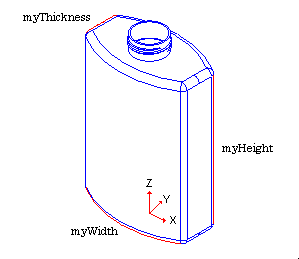
\includegraphics[width=240]{tutorial_image002.png}}
\end{center}
\end{DoxyImageNoCaption}


This modeling requires four steps\+:


\begin{DoxyItemize}
\item build the bottle\textquotesingle{}s Profile
\item build the bottle\textquotesingle{}s Body
\item build the Threading on the bottle\textquotesingle{}s neck
\item build the result compound
\end{DoxyItemize}\hypertarget{occt__tutorial_sec2}{}\section{Building the Profile}\label{occt__tutorial_sec2}
\hypertarget{occt__tutorial_OCCT_TUTORIAL_SUB2_1}{}\subsection{Defining Support Points}\label{occt__tutorial_OCCT_TUTORIAL_SUB2_1}
To create the bottle\textquotesingle{}s profile, you first create characteristic points with their coordinates as shown below in the (X\+OY) plane. These points will be the supports that define the geometry of the profile.


\begin{DoxyImageNoCaption}
\begin{center}
   \mbox{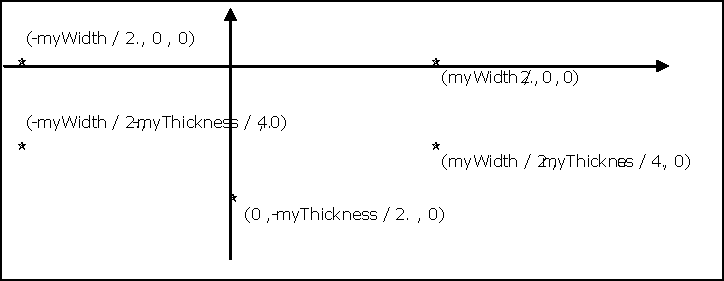
\includegraphics[width=466]{tutorial_image003.pdf}}
\end{center}
\end{DoxyImageNoCaption}


There are two classes to describe a 3D Cartesian point from its X, Y and Z coordinates in Open C\+A\+S\+C\+A\+DE Technology\+:


\begin{DoxyItemize}
\item the primitive geometric {\itshape gp\+\_\+\+Pnt} class
\item the transient {\itshape Geom\+\_\+\+Cartesian\+Point} class manipulated by handle
\end{DoxyItemize}

A handle is a type of smart pointer that provides automatic memory management. To choose the best class for this application, consider the following\+:


\begin{DoxyItemize}
\item {\itshape gp\+\_\+\+Pnt} is manipulated by value. Like all objects of its kind, it will have a limited lifetime.
\item {\itshape Geom\+\_\+\+Cartesian\+Point} is manipulated by handle and may have multiple references and a long lifetime.
\end{DoxyItemize}

Since all the points you will define are only used to create the profile\textquotesingle{}s curves, an object with a limited lifetime will do. Choose the {\itshape gp\+\_\+\+Pnt} class. To instantiate a {\itshape gp\+\_\+\+Pnt} object, just specify the X, Y, and Z coordinates of the points in the global Cartesian coordinate system\+:


\begin{DoxyCode}
gp\_Pnt aPnt1(-myWidth / 2., 0, 0);
gp\_Pnt aPnt2(-myWidth / 2., -myThickness / 4., 0);
gp\_Pnt aPnt3(0, -myThickness / 2., 0);
gp\_Pnt aPnt4(myWidth / 2., -myThickness / 4., 0);
gp\_Pnt aPnt5(myWidth / 2., 0, 0);
\end{DoxyCode}


Once your objects are instantiated, you can use methods provided by the class to access and modify its data. For example, to get the X coordinate of a point\+:


\begin{DoxyCode}
Standard\_Real xValue1 = aPnt1.X();
\end{DoxyCode}
\hypertarget{occt__tutorial_OCCT_TUTORIAL_SUB2_2}{}\subsection{Profile\+: Defining the Geometry}\label{occt__tutorial_OCCT_TUTORIAL_SUB2_2}
With the help of the previously defined points, you can compute a part of the bottle\textquotesingle{}s profile geometry. As shown in the figure below, it will consist of two segments and one arc.


\begin{DoxyImageNoCaption}
\begin{center}
   \mbox{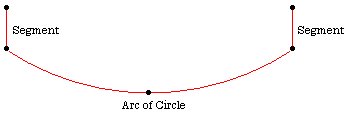
\includegraphics[width=240]{tutorial_image004.png}}
\end{center}
\end{DoxyImageNoCaption}


To create such entities, you need a specific data structure, which implements 3D geometric objects. This can be found in the Geom package of Open C\+A\+S\+C\+A\+DE Technology. In Open C\+A\+S\+C\+A\+DE Technology a package is a group of classes providing related functionality. The classes have names that start with the name of a package they belong to. For example, {\itshape Geom\+\_\+\+Line} and {\itshape Geom\+\_\+\+Circle} classes belong to the {\itshape Geom} package. The {\itshape Geom} package implements 3D geometric objects\+: elementary curves and surfaces are provided as well as more complex ones (such as {\itshape Bezier} and {\itshape B\+Spline}). However, the {\itshape Geom} package provides only the data structure of geometric entities. You can directly instantiate classes belonging to {\itshape Geom}, but it is easier to compute elementary curves and surfaces by using the {\itshape GC} package. This is because the {\itshape GC} provides two algorithm classes which are exactly what is required for our profile\+:


\begin{DoxyItemize}
\item Class {\itshape G\+C\+\_\+\+Make\+Segment} to create a segment. One of its constructors allows you to define a segment by two end points P1 and P2
\item Class {\itshape G\+C\+\_\+\+Make\+Arc\+Of\+Circle} to create an arc of a circle. A useful constructor creates an arc from two end points P1 and P3 and going through P2.
\end{DoxyItemize}

Both of these classes return a {\itshape Geom\+\_\+\+Trimmed\+Curve} manipulated by handle. This entity represents a base curve (line or circle, in our case), limited between two of its parameter values. For example, circle C is parameterized between 0 and 2\+PI. If you need to create a quarter of a circle, you create a {\itshape Geom\+\_\+\+Trimmed\+Curve} on C limited between 0 and M\+\_\+\+P\+I/2.


\begin{DoxyCode}
Handle(Geom\_TrimmedCurve) aArcOfCircle = GC\_MakeArcOfCircle(aPnt2,aPnt3,aPnt4);
Handle(Geom\_TrimmedCurve) aSegment1    = GC\_MakeSegment(aPnt1, aPnt2);
Handle(Geom\_TrimmedCurve) aSegment2    = GC\_MakeSegment(aPnt4, aPnt5);
\end{DoxyCode}


All {\itshape GC} classes provide a casting method to obtain a result automatically with a function-\/like call. Note that this method will raise an exception if construction has failed. To handle possible errors more explicitly, you may use the {\itshape Is\+Done} and {\itshape Value} methods. For example\+:


\begin{DoxyCode}
GC\_MakeSegment mkSeg (aPnt1, aPnt2);
Handle(Geom\_TrimmedCurve) aSegment1;
\textcolor{keywordflow}{if}(mkSegment.IsDone())\{
    aSegment1 = mkSeg.Value();
\}
\textcolor{keywordflow}{else} \{
\textcolor{comment}{// handle error}
\}
\end{DoxyCode}
\hypertarget{occt__tutorial_OCCT_TUTORIAL_SUB2_3}{}\subsection{Profile\+: Defining the Topology}\label{occt__tutorial_OCCT_TUTORIAL_SUB2_3}
You have created the support geometry of one part of the profile but these curves are independent with no relations between each other. To simplify the modeling, it would be right to manipulate these three curves as a single entity. This can be done by using the topological data structure of Open C\+A\+S\+C\+A\+DE Technology defined in the {\itshape Topo\+DS} package\+: it defines relationships between geometric entities which can be linked together to represent complex shapes. Each object of the {\itshape Topo\+DS} package, inheriting from the {\itshape Topo\+D\+S\+\_\+\+Shape} class, describes a topological shape as described below\+:

\tabulinesep=1mm
\begin{longtabu} spread 0pt [c]{*{3}{|X[-1]}|}
\hline
\rowcolor{\tableheadbgcolor}\textbf{ Shape }&\textbf{ Open C\+A\+S\+C\+A\+DE Technology Class }&\textbf{ Description  }\\\cline{1-3}
\endfirsthead
\hline
\endfoot
\hline
\rowcolor{\tableheadbgcolor}\textbf{ Shape }&\textbf{ Open C\+A\+S\+C\+A\+DE Technology Class }&\textbf{ Description  }\\\cline{1-3}
\endhead
Vertex &Topo\+D\+S\+\_\+\+Vertex &Zero dimensional shape corresponding to a point in geometry. \\\cline{1-3}
Edge &Topo\+D\+S\+\_\+\+Edge &One-\/dimensional shape corresponding to a curve and bounded by a vertex at each extremity. \\\cline{1-3}
Wire &Topo\+D\+S\+\_\+\+Wire &Sequence of edges connected by vertices. \\\cline{1-3}
Face &Topo\+D\+S\+\_\+\+Face &Part of a surface bounded by a closed wire(s). \\\cline{1-3}
Shell &Topo\+D\+S\+\_\+\+Shell &Set of faces connected by edges. \\\cline{1-3}
Solid &Topo\+D\+S\+\_\+\+Solid &Part of 3D space bounded by Shells. \\\cline{1-3}
Comp\+Solid &Topo\+D\+S\+\_\+\+Comp\+Solid &Set of solids connected by their faces. \\\cline{1-3}
Compound &Topo\+D\+S\+\_\+\+Compound &Set of any other shapes described above. \\\cline{1-3}
\end{longtabu}
Referring to the previous table, to build the profile, you will create\+:


\begin{DoxyItemize}
\item Three edges out of the previously computed curves.
\item One wire with these edges.
\end{DoxyItemize}


\begin{DoxyImageNoCaption}
\begin{center}
   \mbox{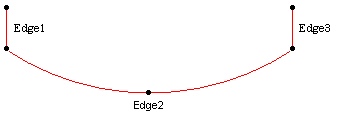
\includegraphics[width=240]{tutorial_image005.png}}
\end{center}
\end{DoxyImageNoCaption}


However, the {\itshape Topo\+DS} package provides only the data structure of the topological entities. Algorithm classes available to compute standard topological objects can be found in the {\itshape B\+Rep\+Builder\+A\+PI} package. To create an edge, you use the B\+Rep\+Builder\+A\+P\+I\+\_\+\+Make\+Edge class with the previously computed curves\+:


\begin{DoxyCode}
TopoDS\_Edge aEdge1 = BRepBuilderAPI\_MakeEdge(aSegment1);
TopoDS\_Edge aEdge2 = BRepBuilderAPI\_MakeEdge(aArcOfCircle);
TopoDS\_Edge aEdge3 = BRepBuilderAPI\_MakeEdge(aSegment2);
\end{DoxyCode}


In Open C\+A\+S\+C\+A\+DE Technology, you can create edges in several ways. One possibility is to create an edge directly from two points, in which case the underlying geometry of this edge is a line, bounded by two vertices being automatically computed from the two input points. For example, a\+Edge1 and a\+Edge3 could have been computed in a simpler way\+:


\begin{DoxyCode}
TopoDS\_Edge aEdge1 = BRepBuilderAPI\_MakeEdge(aPnt1, aPnt3);
TopoDS\_Edge aEdge2 = BRepBuilderAPI\_MakeEdge(aPnt4, aPnt5);
\end{DoxyCode}


To connect the edges, you need to create a wire with the {\itshape B\+Rep\+Builder\+A\+P\+I\+\_\+\+Make\+Wire} class. There are two ways of building a wire with this class\+:


\begin{DoxyItemize}
\item directly from one to four edges
\item by adding other wire(s) or edge(s) to an existing wire (this is explained later in this tutorial)
\end{DoxyItemize}

When building a wire from less than four edges, as in the present case, you can use the constructor directly as follows\+:


\begin{DoxyCode}
TopoDS\_Wire aWire = BRepBuilderAPI\_MakeWire(aEdge1, aEdge2, aEdge3);
\end{DoxyCode}
\hypertarget{occt__tutorial_OCCT_TUTORIAL_SUB2_4}{}\subsection{Profile\+: Completing the Profile}\label{occt__tutorial_OCCT_TUTORIAL_SUB2_4}
Once the first part of your wire is created you need to compute the complete profile. A simple way to do this is to\+:


\begin{DoxyItemize}
\item compute a new wire by reflecting the existing one.
\item add the reflected wire to the initial one.
\end{DoxyItemize}


\begin{DoxyImageNoCaption}
\begin{center}
   \mbox{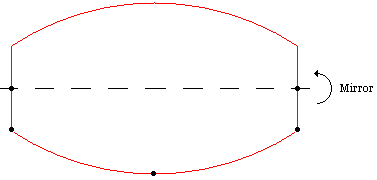
\includegraphics[width=377]{tutorial_image006.png}}
\end{center}
\end{DoxyImageNoCaption}


To apply a transformation on shapes (including wires), you first need to define the properties of a 3D geometric transformation by using the gp\+\_\+\+Trsf class. This transformation can be a translation, a rotation, a scale, a reflection, or a combination of these. In our case, we need to define a reflection with respect to the X axis of the global coordinate system. An axis, defined with the gp\+\_\+\+Ax1 class, is built out of a point and has a direction (3D unitary vector). There are two ways to define this axis. The first way is to define it from scratch, using its geometric definition\+:


\begin{DoxyItemize}
\item X axis is located at (0, 0, 0) -\/ use the {\itshape gp\+\_\+\+Pnt} class.
\item X axis direction is (1, 0, 0) -\/ use the {\itshape gp\+\_\+\+Dir} class. A {\itshape gp\+\_\+\+Dir} instance is created out of its X, Y and Z coordinates.
\end{DoxyItemize}


\begin{DoxyCode}
gp\_Pnt aOrigin(0, 0, 0);
gp\_Dir xDir(1, 0, 0);
gp\_Ax1 xAxis(aOrigin, xDir);
\end{DoxyCode}


The second and simplest way is to use the geometric constants defined in the gp package (origin, main directions and axis of the global coordinate system). To get the X axis, just call the {\itshape gp\+::\+OX} method\+:


\begin{DoxyCode}
gp\_Ax1 xAxis = gp::OX();
\end{DoxyCode}


As previously explained, the 3D geometric transformation is defined with the {\itshape gp\+\_\+\+Trsf} class. There are two different ways to use this class\+:


\begin{DoxyItemize}
\item by defining a transformation matrix by all its values
\item by using the appropriate methods corresponding to the required transformation (Set\+Translation for a translation, Set\+Mirror for a reflection, etc.)\+: the matrix is automatically computed.
\end{DoxyItemize}

Since the simplest approach is always the best one, you should use the Set\+Mirror method with the axis as the center of symmetry.


\begin{DoxyCode}
gp\_Trsf aTrsf;
aTrsf.SetMirror(xAxis);
\end{DoxyCode}


You now have all necessary data to apply the transformation with the B\+Rep\+Builder\+A\+P\+I\+\_\+\+Transform class by specifying\+:


\begin{DoxyItemize}
\item the shape on which the transformation must be applied.
\item the geometric transformation
\end{DoxyItemize}


\begin{DoxyCode}
BRepBuilderAPI\_Transform aBRepTrsf(aWire, aTrsf);
\end{DoxyCode}


{\itshape B\+Rep\+Builder\+A\+P\+I\+\_\+\+Transform} does not modify the nature of the shape\+: the result of the reflected wire remains a wire. But the function-\/like call or the {\itshape B\+Rep\+Builder\+A\+P\+I\+\_\+\+Transform\+::\+Shape} method returns a {\itshape Topo\+D\+S\+\_\+\+Shape} object\+:


\begin{DoxyCode}
TopoDS\_Shape aMirroredShape = aBRepTrsf.Shape();
\end{DoxyCode}


What you need is a method to consider the resulting reflected shape as a wire. The {\itshape Topo\+DS} global functions provide this kind of service by casting a shape into its real type. To cast the transformed wire, use the {\itshape Topo\+D\+S\+::\+Wire} method.


\begin{DoxyCode}
TopoDS\_Wire aMirroredWire = TopoDS::Wire(aMirroredShape);
\end{DoxyCode}


The bottle\textquotesingle{}s profile is almost finished. You have created two wires\+: {\itshape a\+Wire} and {\itshape a\+Mirrored\+Wire}. You need to concatenate them to compute a single shape. To do this, you use the {\itshape B\+Rep\+Builder\+A\+P\+I\+\_\+\+Make\+Wire} class as follows\+:


\begin{DoxyItemize}
\item create an instance of {\itshape B\+Rep\+Builder\+A\+P\+I\+\_\+\+Make\+Wire}.
\item add all edges of the two wires by using the {\itshape Add} method on this object.
\end{DoxyItemize}


\begin{DoxyCode}
BRepBuilderAPI\_MakeWire mkWire;
mkWire.Add(aWire);
mkWire.Add(aMirroredWire);
TopoDS\_Wire myWireProfile = mkWire.Wire();
\end{DoxyCode}
\hypertarget{occt__tutorial_sec3}{}\section{Building the Body}\label{occt__tutorial_sec3}
\hypertarget{occt__tutorial_OCCT_TUTORIAL_SUB3_1}{}\subsection{Prism the Profile}\label{occt__tutorial_OCCT_TUTORIAL_SUB3_1}
To compute the main body of the bottle, you need to create a solid shape. The simplest way is to use the previously created profile and to sweep it along a direction. The {\itshape Prism} functionality of Open C\+A\+S\+C\+A\+DE Technology is the most appropriate for that task. It accepts a shape and a direction as input and generates a new shape according to the following rules\+:

\tabulinesep=1mm
\begin{longtabu} spread 0pt [c]{*{2}{|X[-1]}|}
\hline
\rowcolor{\tableheadbgcolor}\textbf{ Shape }&\textbf{ Generates  }\\\cline{1-2}
\endfirsthead
\hline
\endfoot
\hline
\rowcolor{\tableheadbgcolor}\textbf{ Shape }&\textbf{ Generates  }\\\cline{1-2}
\endhead
Vertex &Edge \\\cline{1-2}
Edge &Face \\\cline{1-2}
Wire &Shell \\\cline{1-2}
Face &Solid \\\cline{1-2}
Shell &Compound of Solids \\\cline{1-2}
\end{longtabu}

\begin{DoxyImageNoCaption}
\begin{center}
   \mbox{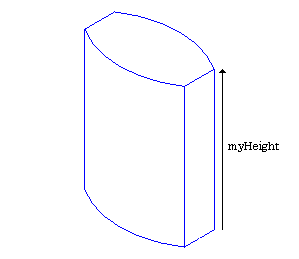
\includegraphics[width=240]{tutorial_image007.png}}
\end{center}
\end{DoxyImageNoCaption}


Your current profile is a wire. Referring to the Shape/\+Generates table, you need to compute a face out of its wire to generate a solid. To create a face, use the {\itshape B\+Rep\+Builder\+A\+P\+I\+\_\+\+Make\+Face} class. As previously explained, a face is a part of a surface bounded by a closed wire. Generally, {\itshape B\+Rep\+Builder\+A\+P\+I\+\_\+\+Make\+Face} computes a face out of a surface and one or more wires. When the wire lies on a plane, the surface is automatically computed.


\begin{DoxyCode}
TopoDS\_Face myFaceProfile = BRepBuilderAPI\_MakeFace(myWireProfile);
\end{DoxyCode}


The {\itshape B\+Rep\+Prim\+A\+PI} package provides all the classes to create topological primitive constructions\+: boxes, cones, cylinders, spheres, etc. Among them is the {\itshape B\+Rep\+Prim\+A\+P\+I\+\_\+\+Make\+Prism} class. As specified above, the prism is defined by\+:


\begin{DoxyItemize}
\item the basis shape to sweep;
\item a vector for a finite prism or a direction for finite and infinite prisms.
\end{DoxyItemize}

You want the solid to be finite, swept along the Z axis and to be my\+Height height. The vector, defined with the {\itshape gp\+\_\+\+Vec} class on its X, Y and Z coordinates, is\+:


\begin{DoxyCode}
gp\_Vec aPrismVec(0, 0, myHeight);
\end{DoxyCode}


All the necessary data to create the main body of your bottle is now available. Just apply the {\itshape B\+Rep\+Prim\+A\+P\+I\+\_\+\+Make\+Prism} class to compute the solid\+:


\begin{DoxyCode}
TopoDS\_Shape myBody = BRepPrimAPI\_MakePrism(myFaceProfile, aPrismVec);
\end{DoxyCode}
\hypertarget{occt__tutorial_OCCT_TUTORIAL_SUB3_2}{}\subsection{Applying Fillets}\label{occt__tutorial_OCCT_TUTORIAL_SUB3_2}
The edges of the bottle\textquotesingle{}s body are very sharp. To replace them by rounded faces, you use the {\itshape Fillet} functionality of Open C\+A\+S\+C\+A\+DE Technology. For our purposes, we will specify that fillets must be\+:


\begin{DoxyItemize}
\item applied on all edges of the shape
\item have a radius of {\itshape my\+Thickness} / 12
\end{DoxyItemize}


\begin{DoxyImageNoCaption}
\begin{center}
   \mbox{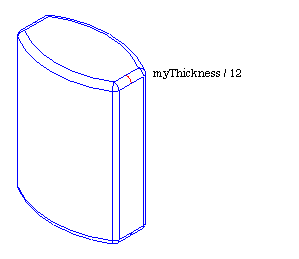
\includegraphics[width=240]{tutorial_image008.png}}
\end{center}
\end{DoxyImageNoCaption}


To apply fillets on the edges of a shape, you use the {\itshape B\+Rep\+Fillet\+A\+P\+I\+\_\+\+Make\+Fillet} class. This class is normally used as follows\+:


\begin{DoxyItemize}
\item Specify the shape to be filleted in the {\itshape B\+Rep\+Fillet\+A\+P\+I\+\_\+\+Make\+Fillet} constructor.
\item Add the fillet descriptions (an edge and a radius) using the {\itshape Add} method (you can add as many edges as you need).
\item Ask for the resulting filleted shape with the {\itshape Shape} method.
\end{DoxyItemize}


\begin{DoxyCode}
BRepFilletAPI\_MakeFillet mkFillet(myBody);
\end{DoxyCode}


To add the fillet description, you need to know the edges belonging to your shape. The best solution is to explore your solid to retrieve its edges. This kind of functionality is provided with the {\itshape Top\+Exp\+\_\+\+Explorer} class, which explores the data structure described in a {\itshape Topo\+D\+S\+\_\+\+Shape} and extracts the sub-\/shapes you specifically need. Generally, this explorer is created by providing the following information\+:


\begin{DoxyItemize}
\item the shape to explore
\item the type of sub-\/shapes to be found. This information is given with the {\itshape Top\+Abs\+\_\+\+Shape\+Enum} enumeration.
\end{DoxyItemize}


\begin{DoxyCode}
TopExp\_Explorer anEdgeExplorer(myBody, TopAbs\_EDGE);
\end{DoxyCode}


An explorer is usually applied in a loop by using its three main methods\+:


\begin{DoxyItemize}
\item {\itshape More()} to know if there are more sub-\/shapes to explore.
\item {\itshape Current()} to know which is the currently explored sub-\/shape (used only if the {\itshape More()} method returns true).
\item {\itshape Next()} to move onto the next sub-\/shape to explore.
\end{DoxyItemize}


\begin{DoxyCode}
\textcolor{keywordflow}{while}(anEdgeExplorer.More())\{
    TopoDS\_Edge anEdge = TopoDS::Edge(anEdgeExplorer.Current());
    \textcolor{comment}{//Add edge to fillet algorithm}
    ...
    anEdgeExplorer.Next();
\}
\end{DoxyCode}


In the explorer loop, you have found all the edges of the bottle shape. Each one must then be added in the {\itshape B\+Rep\+Fillet\+A\+P\+I\+\_\+\+Make\+Fillet} instance with the {\itshape Add()} method. Do not forget to specify the radius of the fillet along with it.


\begin{DoxyCode}
mkFillet.Add(myThickness / 12., anEdge);
\end{DoxyCode}


Once this is done, you perform the last step of the procedure by asking for the filleted shape.


\begin{DoxyCode}
myBody = mkFillet.Shape();
\end{DoxyCode}
\hypertarget{occt__tutorial_OCCT_TUTORIAL_SUB3_3}{}\subsection{Adding the Neck}\label{occt__tutorial_OCCT_TUTORIAL_SUB3_3}
To add a neck to the bottle, you will create a cylinder and fuse it to the body. The cylinder is to be positioned on the top face of the body with a radius of {\itshape my\+Thickness} / 4. and a height of {\itshape my\+Height} / 10.


\begin{DoxyImageNoCaption}
\begin{center}
   \mbox{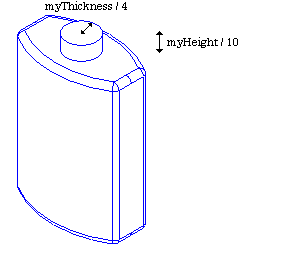
\includegraphics[width=240]{tutorial_image009.png}}
\end{center}
\end{DoxyImageNoCaption}


To position the cylinder, you need to define a coordinate system with the {\itshape gp\+\_\+\+Ax2} class defining a right-\/handed coordinate system from a point and two directions -\/ the main (Z) axis direction and the X direction (the Y direction is computed from these two). To align the neck with the center of the top face, being in the global coordinate system (0, 0, {\itshape my\+Height}), with its normal on the global Z axis, your local coordinate system can be defined as follows\+:


\begin{DoxyCode}
gp\_Pnt neckLocation(0, 0, myHeight);
gp\_Dir neckAxis = gp::DZ();
gp\_Ax2 neckAx2(neckLocation, neckAxis);
\end{DoxyCode}


To create a cylinder, use another class from the primitives construction package\+: the {\itshape B\+Rep\+Prim\+A\+P\+I\+\_\+\+Make\+Cylinder} class. The information you must provide is\+:


\begin{DoxyItemize}
\item the coordinate system where the cylinder will be located;
\item the radius and height.
\end{DoxyItemize}


\begin{DoxyCode}
Standard\_Real myNeckRadius = myThickness / 4.;
Standard\_Real myNeckHeight = myHeight / 10;
BRepPrimAPI\_MakeCylinder MKCylinder(neckAx2, myNeckRadius, myNeckHeight);
TopoDS\_Shape myNeck = MKCylinder.Shape();
\end{DoxyCode}


You now have two separate parts\+: a main body and a neck that you need to fuse together. The {\itshape B\+Rep\+Algo\+A\+PI} package provides services to perform Boolean operations between shapes, and especially\+: {\itshape common} (Boolean intersection), {\itshape cut} (Boolean subtraction) and {\itshape fuse} (Boolean union). Use {\itshape B\+Rep\+Algo\+A\+P\+I\+\_\+\+Fuse} to fuse the two shapes\+:


\begin{DoxyCode}
myBody = BRepAlgoAPI\_Fuse(myBody, myNeck);
\end{DoxyCode}
\hypertarget{occt__tutorial_OCCT_TUTORIAL_SUB3_4}{}\subsection{Creating a Hollowed Solid}\label{occt__tutorial_OCCT_TUTORIAL_SUB3_4}
Since a real bottle is used to contain liquid material, you should now create a hollowed solid from the bottle\textquotesingle{}s top face. In Open C\+A\+S\+C\+A\+DE Technology, a hollowed solid is called a {\itshape Thick} {\itshape Solid} and is internally computed as follows\+:


\begin{DoxyItemize}
\item Remove one or more faces from the initial solid to obtain the first wall W1 of the hollowed solid.
\item Create a parallel wall W2 from W1 at a distance D. If D is positive, W2 will be outside the initial solid, otherwise it will be inside.
\item Compute a solid from the two walls W1 and W2.
\end{DoxyItemize}


\begin{DoxyImageNoCaption}
\begin{center}
   \mbox{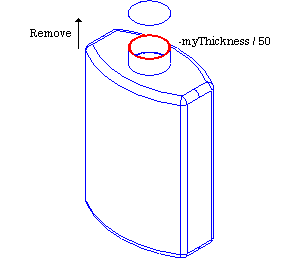
\includegraphics[width=240]{tutorial_image010.png}}
\end{center}
\end{DoxyImageNoCaption}


To compute a thick solid, you create an instance of the {\itshape B\+Rep\+Offset\+A\+P\+I\+\_\+\+Make\+Thick\+Solid} class by giving the following information\+:


\begin{DoxyItemize}
\item The shape, which must be hollowed.
\item The tolerance used for the computation (tolerance criterion for coincidence in generated shapes).
\item The thickness between the two walls W1 and W2 (distance D).
\item The face(s) to be removed from the original solid to compute the first wall W1.
\end{DoxyItemize}

The challenging part in this procedure is to find the face to remove from your shape -\/ the top face of the neck, which\+:


\begin{DoxyItemize}
\item has a plane (planar surface) as underlying geometry;
\item is the highest face (in Z coordinates) of the bottle.
\end{DoxyItemize}

To find the face with such characteristics, you will once again use an explorer to iterate on all the bottle\textquotesingle{}s faces to find the appropriate one.


\begin{DoxyCode}
\textcolor{keywordflow}{for}(TopExp\_Explorer aFaceExplorer(myBody, TopAbs\_FACE) ; aFaceExplorer.More() ; aFaceExplorer.Next())\{
    TopoDS\_Face aFace = TopoDS::Face(aFaceExplorer.Current());
\}
\end{DoxyCode}


For each detected face, you need to access the geometric properties of the shape\+: use the {\itshape B\+Rep\+\_\+\+Tool} class for that. The most commonly used methods of this class are\+:


\begin{DoxyItemize}
\item {\itshape Surface} to access the surface of a face;
\item {\itshape Curve} to access the 3D curve of an edge;
\item {\itshape Point} to access the 3D point of a vertex.
\end{DoxyItemize}


\begin{DoxyCode}
Handle(Geom\_Surface) aSurface = BRep\_Tool::Surface(aFace);
\end{DoxyCode}


As you can see, the {\itshape B\+Rep\+\_\+\+Tool\+::\+Surface} method returns an instance of the {\itshape Geom\+\_\+\+Surface} class manipulated by handle. However, the {\itshape Geom\+\_\+\+Surface} class does not provide information about the real type of the object {\itshape a\+Surface}, which could be an instance of {\itshape Geom\+\_\+\+Plane}, {\itshape Geom\+\_\+\+Cylindrical\+Surface}, etc. All objects manipulated by handle, like {\itshape Geom\+\_\+\+Surface}, inherit from the {\itshape Standard\+\_\+\+Transient} class which provides two very useful methods concerning types\+:


\begin{DoxyItemize}
\item {\itshape Dynamic\+Type} to know the real type of the object
\item {\itshape Is\+Kind} to know if the object inherits from one particular type
\end{DoxyItemize}

Dynamic\+Type returns the real type of the object, but you need to compare it with the existing known types to determine whether {\itshape a\+Surface} is a plane, a cylindrical surface or some other type. To compare a given type with the type you seek, use the {\itshape S\+T\+A\+N\+D\+A\+R\+D\+\_\+\+T\+Y\+PE} macro, which returns the type of a class\+:


\begin{DoxyCode}
\textcolor{keywordflow}{if}(aSurface->DynamicType() == STANDARD\_TYPE(Geom\_Plane))\{
\textcolor{comment}{//}
\}
\end{DoxyCode}


If this comparison is true, you know that the {\itshape a\+Surface} real type is {\itshape Geom\+\_\+\+Plane}. You can then convert it from {\itshape Geom\+\_\+\+Surface} to {\itshape Geom\+\_\+\+Plane} by using the {\itshape Down\+Cast()} method provided by each class inheriting {\itshape Standard\+\_\+\+Transient}. As its name implies, this static method is used to downcast objects to a given type with the following syntax\+:


\begin{DoxyCode}
Handle(Geom\_Plane) aPlane = Handle(Geom\_Plane)::DownCast(aSurface);
\end{DoxyCode}


Remember that the goal of all these conversions is to find the highest face of the bottle lying on a plane. Suppose that you have these two global variables\+:


\begin{DoxyCode}
TopoDS\_Face faceToRemove;
Standard\_Real zMax = -1;
\end{DoxyCode}


You can easily find the plane whose origin is the biggest in Z knowing that the location of the plane is given with the {\itshape Geom\+\_\+\+Plane\+::\+Location} method. For example\+:


\begin{DoxyCode}
gp\_Pnt aPnt = aPlane->Location();
Standard\_Real aZ = aPnt.Z();
\textcolor{keywordflow}{if}(aZ > zMax)\{
    zMax = aZ;
    faceToRemove = aFace;
\}
\end{DoxyCode}


You have now found the top face of the neck. Your final step before creating the hollowed solid is to put this face in a list. Since more than one face can be removed from the initial solid, the {\itshape B\+Rep\+Offset\+A\+P\+I\+\_\+\+Make\+Thick\+Solid} constructor takes a list of faces as arguments. Open C\+A\+S\+C\+A\+DE Technology provides many collections for different kinds of objects\+: see {\itshape T\+Col\+Geom} package for collections of objects from {\itshape Geom} package, {\itshape T\+Colgp} package for collections of objects from gp package, etc. The collection for shapes can be found in the {\itshape Top\+Tools} package. As {\itshape B\+Rep\+Offset\+A\+P\+I\+\_\+\+Make\+Thick\+Solid} requires a list, use the {\itshape Top\+Tools\+\_\+\+List\+Of\+Shape} class.


\begin{DoxyCode}
TopTools\_ListOfShape facesToRemove;
facesToRemove.Append(faceToRemove);
\end{DoxyCode}


All the necessary data are now available so you can create your hollowed solid by calling the {\itshape B\+Rep\+Offset\+A\+P\+I\+\_\+\+Make\+Thick\+Solid} Make\+Thick\+Solid\+By\+Join method\+:


\begin{DoxyCode}
BRepOffsetAPI\_MakeThickSolid BodyMaker;
BodyMaker.MakeThickSolidByJoin(myBody, facesToRemove, -myThickness / 50, 1.e-3);
myBody = BodyMaker.Shape();
\end{DoxyCode}
\hypertarget{occt__tutorial_sec4}{}\section{Building the Threading}\label{occt__tutorial_sec4}
\hypertarget{occt__tutorial_OCCT_TUTORIAL_SUB4_1}{}\subsection{Creating Surfaces}\label{occt__tutorial_OCCT_TUTORIAL_SUB4_1}
Up to now, you have learned how to create edges out of 3D curves. You will now learn how to create an edge out of a 2D curve and a surface. To learn this aspect of Open C\+A\+S\+C\+A\+DE Technology, you will build helicoidal profiles out of 2D curves on cylindrical surfaces. The theory is more complex than in previous steps, but applying it is very simple. As a first step, you compute these cylindrical surfaces. You are already familiar with curves of the {\itshape Geom} package. Now you can create a cylindrical surface ({\itshape Geom\+\_\+\+Cylindrical\+Surface}) using\+:


\begin{DoxyItemize}
\item a coordinate system;
\item a radius.
\end{DoxyItemize}

Using the same coordinate system {\itshape neck\+Ax2} used to position the neck, you create two cylindrical surfaces {\itshape Geom\+\_\+\+Cylindrical\+Surface} with the following radii\+:


\begin{DoxyImageNoCaption}
\begin{center}
   \mbox{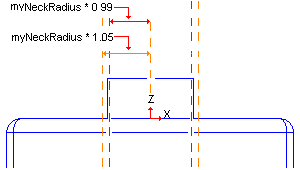
\includegraphics[width=300]{tutorial_image011.png}}
\end{center}
\end{DoxyImageNoCaption}


Notice that one of the cylindrical surfaces is smaller than the neck. There is a good reason for this\+: after the thread creation, you will fuse it with the neck. So, we must make sure that the two shapes remain in contact.


\begin{DoxyCode}
Handle(Geom\_CylindricalSurface) aCyl1 = \textcolor{keyword}{new} Geom\_CylindricalSurface(neckAx2, myNeckRadius * 0.99);

Handle(Geom\_CylindricalSurface) aCyl2 = \textcolor{keyword}{new} Geom\_CylindricalSurface(neckAx2, myNeckRadius * 1.05);
\end{DoxyCode}
\hypertarget{occt__tutorial_OCCT_TUTORIAL_SUB4_2}{}\subsection{Defining 2\+D Curves}\label{occt__tutorial_OCCT_TUTORIAL_SUB4_2}
To create the neck of the bottle, you made a solid cylinder based on a cylindrical surface. You will create the profile of threading by creating 2D curves on such a surface. All geometries defined in the {\itshape Geom} package are parameterized. This means that each curve or surface from Geom is computed with a parametric equation. A {\itshape Geom\+\_\+\+Cylindrical\+Surface} surface is defined with the following parametric equation\+:

P(\+U, V) = O + R $\ast$ (cos(\+U) $\ast$ x\+Dir + sin(\+U) $\ast$ y\+Dir) + V $\ast$ z\+Dir, where \+:


\begin{DoxyItemize}
\item P is the point defined by parameters (U, V).
\item O, $\ast$\+Dir, y\+Dir and z\+Dir are respectively the origin, the X direction, Y direction and Z direction of the cylindrical surface local coordinate system.
\item R is the radius of the cylindrical surface.
\item U range is \mbox{[}0, 2\+PI\mbox{]} and V is infinite.
\end{DoxyItemize}


\begin{DoxyImageNoCaption}
\begin{center}
   \mbox{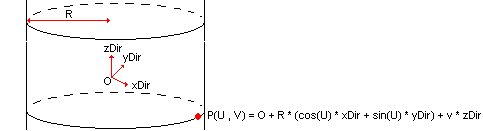
\includegraphics[width=400]{tutorial_image012.png}}
\end{center}
\end{DoxyImageNoCaption}


The advantage of having such parameterized geometries is that you can compute, for any (U, V) parameters of the surface\+:


\begin{DoxyItemize}
\item the 3D point;
\item the derivative vectors of order 1, 2 to N at this point.
\end{DoxyItemize}

There is another advantage of these parametric equations\+: you can consider a surface as a 2D parametric space defined with a (U, V) coordinate system. For example, consider the parametric ranges of the neck\textquotesingle{}s surface\+:


\begin{DoxyImageNoCaption}
\begin{center}
   \mbox{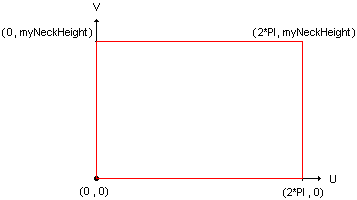
\includegraphics[width=320]{tutorial_image013.png}}
\end{center}
\end{DoxyImageNoCaption}


Suppose that you create a 2D line on this parametric (U, V) space and compute its 3D parametric curve. Depending on the line definition, results are as follows\+:

\tabulinesep=1mm
\begin{longtabu} spread 0pt [c]{*{3}{|X[-1]}|}
\hline
\rowcolor{\tableheadbgcolor}\textbf{ Case }&\textbf{ Parametric Equation }&\textbf{ Parametric Curve  }\\\cline{1-3}
\endfirsthead
\hline
\endfoot
\hline
\rowcolor{\tableheadbgcolor}\textbf{ Case }&\textbf{ Parametric Equation }&\textbf{ Parametric Curve  }\\\cline{1-3}
\endhead
U = 0 &P(\+V) = O + V $\ast$ z\+Dir &Line parallel to the Z direction \\\cline{1-3}
V = 0 &P(\+U) = O + R $\ast$ (cos(\+U) $\ast$ x\+Dir + sin(\+U) $\ast$ y\+Dir) &Circle parallel to the (O, X, Y) plane \\\cline{1-3}
U != 0 V != 0 &P(\+U, V) = O + R $\ast$ (cos(\+U) $\ast$ x\+Dir + sin(\+U) $\ast$ y\+Dir) + V $\ast$ z\+Dir &Helicoidal curve describing the evolution of height and angle on the cylinder \\\cline{1-3}
\end{longtabu}
The helicoidal curve type is exactly what you need. On the neck\textquotesingle{}s surface, the evolution laws of this curve will be\+:


\begin{DoxyItemize}
\item In V parameter\+: between 0 and my\+Heigh\+Neck for the height description
\item In U parameter\+: between 0 and 2\+PI for the angle description. But, since a cylindrical surface is U periodic, you can decide to extend this angle evolution to 4\+PI as shown in the following drawing\+:
\end{DoxyItemize}


\begin{DoxyImageNoCaption}
\begin{center}
   \mbox{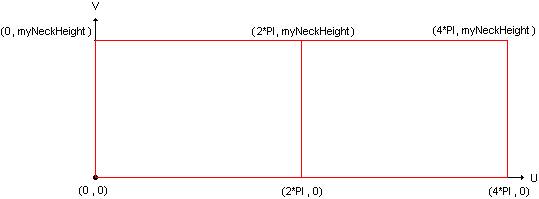
\includegraphics[width=440]{tutorial_image014.png}}
\end{center}
\end{DoxyImageNoCaption}


In this (U, V) parametric space, you will create a local (X, Y) coordinate system to position the curves to be created. This coordinate system will be defined with\+:


\begin{DoxyItemize}
\item A center located in the middle of the neck\textquotesingle{}s cylinder parametric space at (2$\ast$\+PI, my\+Neck\+Height / 2) in U, V coordinates.
\item A X direction defined with the (2$\ast$\+PI, my\+Neck\+Height/4) vector in U, V coordinates, so that the curves occupy half of the neck\textquotesingle{}s surfaces.
\end{DoxyItemize}


\begin{DoxyImageNoCaption}
\begin{center}
   \mbox{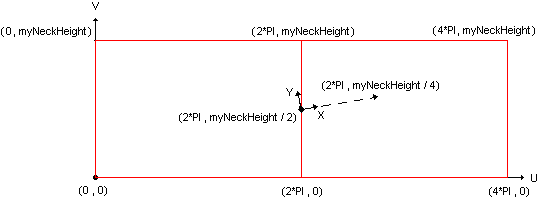
\includegraphics[width=440]{tutorial_image015.png}}
\end{center}
\end{DoxyImageNoCaption}


To use 2D primitive geometry types of Open C\+A\+S\+C\+A\+DE Technology for defining a point and a coordinate system, you will once again instantiate classes from gp\+:


\begin{DoxyItemize}
\item To define a 2D point from its X and Y coordinates, use the {\itshape gp\+\_\+\+Pnt2d} class.
\item To define a 2D direction (unit vector) from its X and Y coordinates, use the gp\+\_\+\+Dir2d class. The coordinates will automatically be normalized.
\item To define a 2D right-\/handed coordinate system, use the {\itshape gp\+\_\+\+Ax2d} class, which is computed from a point (origin of the coordinate system) and a direction -\/ the X direction of the coordinate system. The Y direction will be automatically computed.
\end{DoxyItemize}


\begin{DoxyCode}
gp\_Pnt2d aPnt(2. * M\_PI, myNeckHeight / 2.);
gp\_Dir2d aDir(2. * M\_PI, myNeckHeight / 4.);
gp\_Ax2d anAx2d(aPnt, aDir);
\end{DoxyCode}


You will now define the curves. As previously mentioned, these thread profiles are computed on two cylindrical surfaces. In the following figure, curves on the left define the base (on {\itshape a\+Cyl1} surface) and the curves on the right define the top of the thread\textquotesingle{}s shape (on {\itshape a\+Cyl2} surface).


\begin{DoxyImageNoCaption}
\begin{center}
   \mbox{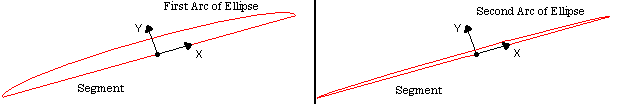
\includegraphics[width=440]{tutorial_image016.png}}
\end{center}
\end{DoxyImageNoCaption}


You have already used the {\itshape Geom} package to define 3D geometric entities. For 2D, you will use the {\itshape Geom2d} package. As for {\itshape Geom}, all geometries are parameterized. For example, a {\itshape Geom2d\+\_\+\+Ellipse} ellipse is defined from\+:


\begin{DoxyItemize}
\item a coordinate system whose origin is the ellipse center;
\item a major radius on the major axis defined by the X direction of the coordinate system;
\item a minor radius on the minor axis defined by the Y direction of the coordinate system.
\end{DoxyItemize}

Supposing that\+:


\begin{DoxyItemize}
\item Both ellipses have the same major radius of 2$\ast$\+PI,
\item Minor radius of the first ellipse is my\+Neck\+Height / 10,
\item And the minor radius value of the second ellipse is a fourth of the first one,
\end{DoxyItemize}

Your ellipses are defined as follows\+:


\begin{DoxyCode}
Standard\_Real aMajor = 2. * M\_PI;
Standard\_Real aMinor = myNeckHeight / 10;
Handle(Geom2d\_Ellipse) anEllipse1 = \textcolor{keyword}{new} Geom2d\_Ellipse(anAx2d, aMajor, aMinor);
Handle(Geom2d\_Ellipse) anEllipse2 = \textcolor{keyword}{new} Geom2d\_Ellipse(anAx2d, aMajor, aMinor / 4);
\end{DoxyCode}


To describe portions of curves for the arcs drawn above, you define {\itshape Geom2d\+\_\+\+Trimmed\+Curve} trimmed curves out of the created ellipses and two parameters to limit them. As the parametric equation of an ellipse is P(\+U) = O + (Major\+Radius $\ast$ cos(\+U) $\ast$ X\+Direction) + (Minor\+Radius $\ast$ sin(\+U) $\ast$ Y\+Direction), the ellipses need to be limited between 0 and M\+\_\+\+PI.


\begin{DoxyCode}
Handle(Geom2d\_TrimmedCurve) anArc1 = \textcolor{keyword}{new} Geom2d\_TrimmedCurve(anEllipse1, 0, M\_PI);
Handle(Geom2d\_TrimmedCurve) anArc2 = \textcolor{keyword}{new} Geom2d\_TrimmedCurve(anEllipse2, 0, M\_PI);
\end{DoxyCode}


The last step consists in defining the segment, which is the same for the two profiles\+: a line limited by the first and the last point of one of the arcs. To access the point corresponding to the parameter of a curve or a surface, you use the Value or D0 method (meaning 0th derivative), D1 method is for first derivative, D2 for the second one.


\begin{DoxyCode}
gp\_Pnt2d anEllipsePnt1 = anEllipse1->Value(0);
gp\_Pnt2d anEllipsePnt2;
anEllipse1->D0(M\_PI, anEllipsePnt2);
\end{DoxyCode}


When creating the bottle\textquotesingle{}s profile, you used classes from the {\itshape GC} package, providing algorithms to create elementary geometries. In 2D geometry, this kind of algorithms is found in the {\itshape G\+C\+E2d} package. Class names and behaviors are similar to those in {\itshape GC}. For example, to create a 2D segment out of two points\+:


\begin{DoxyCode}
Handle(Geom2d\_TrimmedCurve) aSegment = GCE2d\_MakeSegment(anEllipsePnt1, anEllipsePnt2);
\end{DoxyCode}
\hypertarget{occt__tutorial_OCCT_TUTORIAL_SUB4_3}{}\subsection{Building Edges and Wires}\label{occt__tutorial_OCCT_TUTORIAL_SUB4_3}
As you did when creating the base profile of the bottle, you can now\+:


\begin{DoxyItemize}
\item compute the edges of the neck\textquotesingle{}s threading.
\item compute two wires out of these edges.
\end{DoxyItemize}


\begin{DoxyImageNoCaption}
\begin{center}
   \mbox{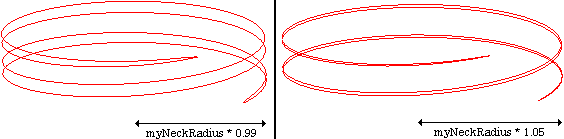
\includegraphics[width=440]{tutorial_image017.png}}
\end{center}
\end{DoxyImageNoCaption}


Previously, you have built\+:


\begin{DoxyItemize}
\item two cylindrical surfaces of the threading
\item three 2D curves defining the base geometry of the threading
\end{DoxyItemize}

To compute the edges out of these curves, once again use the {\itshape B\+Rep\+Builder\+A\+P\+I\+\_\+\+Make\+Edge} class. One of its constructors allows you to build an edge out of a curve described in the 2D parametric space of a surface.


\begin{DoxyCode}
TopoDS\_Edge anEdge1OnSurf1 = BRepBuilderAPI\_MakeEdge(anArc1, aCyl1);
TopoDS\_Edge anEdge2OnSurf1 = BRepBuilderAPI\_MakeEdge(aSegment, aCyl1);
TopoDS\_Edge anEdge1OnSurf2 = BRepBuilderAPI\_MakeEdge(anArc2, aCyl2);
TopoDS\_Edge anEdge2OnSurf2 = BRepBuilderAPI\_MakeEdge(aSegment, aCyl2);
\end{DoxyCode}


Now, you can create the two profiles of the threading, lying on each surface.


\begin{DoxyCode}
TopoDS\_Wire threadingWire1 = BRepBuilderAPI\_MakeWire(anEdge1OnSurf1, anEdge2OnSurf1);
TopoDS\_Wire threadingWire2 = BRepBuilderAPI\_MakeWire(anEdge1OnSurf2, anEdge2OnSurf2);
\end{DoxyCode}


Remember that these wires were built out of a surface and 2D curves. One important data item is missing as far as these wires are concerned\+: there is no information on the 3D curves. Fortunately, you do not need to compute this yourself, which can be a difficult task since the mathematics can be quite complex. When a shape contains all the necessary information except 3D curves, Open C\+A\+S\+C\+A\+DE Technology provides a tool to build them automatically. In the B\+Rep\+Lib tool package, you can use the {\itshape Build\+Curves3d} method to compute 3D curves for all the edges of a shape.


\begin{DoxyCode}
BRepLib::BuildCurves3d(threadingWire1);
BRepLib::BuildCurves3d(threadingWire2);
\end{DoxyCode}
\hypertarget{occt__tutorial_OCCT_TUTORIAL_SUB4_4}{}\subsection{Creating Threading}\label{occt__tutorial_OCCT_TUTORIAL_SUB4_4}
You have computed the wires of the threading. The threading will be a solid shape, so you must now compute the faces of the wires, the faces allowing you to join the wires, the shell out of these faces and then the solid itself. This can be a lengthy operation. There are always faster ways to build a solid when the base topology is defined. You would like to create a solid out of two wires. Open C\+A\+S\+C\+A\+DE Technology provides a quick way to do this by building a loft\+: a shell or a solid passing through a set of wires in a given sequence. The loft function is implemented in the {\itshape B\+Rep\+Offset\+A\+P\+I\+\_\+\+Thru\+Sections} class, which you use as follows\+:


\begin{DoxyImageNoCaption}
\begin{center}
   \mbox{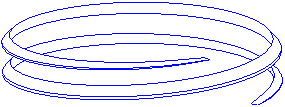
\includegraphics[width=285]{tutorial_image018.png}}
\end{center}
\end{DoxyImageNoCaption}



\begin{DoxyItemize}
\item Initialize the algorithm by creating an instance of the class. The first parameter of this constructor must be specified if you want to create a solid. By default, {\itshape B\+Rep\+Offset\+A\+P\+I\+\_\+\+Thru\+Sections} builds a shell.
\item Add the successive wires using the Add\+Wire method.
\item Use the {\itshape Check\+Compatibility} method to activate (or deactivate) the option that checks whether the wires have the same number of edges. In this case, wires have two edges each, so you can deactivate this option.
\item Ask for the resulting loft shape with the Shape method.
\end{DoxyItemize}


\begin{DoxyCode}
BRepOffsetAPI\_ThruSections aTool(Standard\_True);
aTool.AddWire(threadingWire1); aTool.AddWire(threadingWire2);
aTool.CheckCompatibility(Standard\_False);
TopoDS\_Shape myThreading = aTool.Shape();
\end{DoxyCode}
\hypertarget{occt__tutorial_sec5}{}\section{Building the Resulting Compound}\label{occt__tutorial_sec5}
You are almost done building the bottle. Use the {\itshape Topo\+D\+S\+\_\+\+Compound} and {\itshape B\+Rep\+\_\+\+Builder} classes to build single shape from {\itshape my\+Body} and {\itshape my\+Threading}\+:


\begin{DoxyCode}
TopoDS\_Compound aRes;
BRep\_Builder aBuilder;
aBuilder.MakeCompound (aRes);
aBuilder.Add (aRes, myBody);
aBuilder.Add (aRes, myThreading);
\end{DoxyCode}


Congratulations! Your bottle is complete. Here is the result snapshot of the Tutorial application\+:


\begin{DoxyImageNoCaption}
\begin{center}
   \mbox{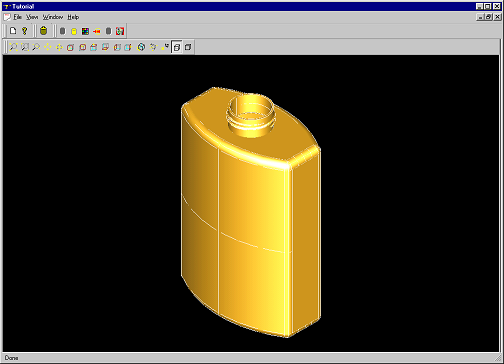
\includegraphics[width=320]{tutorial_image019.png}}
\end{center}
\end{DoxyImageNoCaption}


We hope that this tutorial has provided you with a feel for the industrial strength power of Open C\+A\+S\+C\+A\+DE Technology. If you want to know more and develop major projects using Open C\+A\+S\+C\+A\+DE Technology, we invite you to study our training, support, and consulting services on our site at \href{http://www.opencascade.com/content/technology-support}{\tt http\+://www.\+opencascade.\+com/content/technology-\/support}. Our professional services can maximize the power of your Open C\+A\+S\+C\+A\+DE Technology applications.\hypertarget{occt__tutorial_sec6}{}\section{Appendix}\label{occt__tutorial_sec6}
Complete definition of Make\+Bottle function (defined in the file src/\+Make\+Bottle.\+cxx of the Tutorial)\+:


\begin{DoxyCode}
TopoDS\_Shape MakeBottle(\textcolor{keyword}{const} Standard\_Real myWidth, \textcolor{keyword}{const} Standard\_Real myHeight,
                        \textcolor{keyword}{const} Standard\_Real myThickness)
\{
    \textcolor{comment}{// Profile : Define Support Points}
    gp\_Pnt aPnt1(-myWidth / 2., 0, 0);        
    gp\_Pnt aPnt2(-myWidth / 2., -myThickness / 4., 0);
    gp\_Pnt aPnt3(0, -myThickness / 2., 0);
    gp\_Pnt aPnt4(myWidth / 2., -myThickness / 4., 0);
    gp\_Pnt aPnt5(myWidth / 2., 0, 0);

    \textcolor{comment}{// Profile : Define the Geometry}
    Handle(Geom\_TrimmedCurve) anArcOfCircle = GC\_MakeArcOfCircle(aPnt2,aPnt3,aPnt4);
    Handle(Geom\_TrimmedCurve) aSegment1 = GC\_MakeSegment(aPnt1, aPnt2);
    Handle(Geom\_TrimmedCurve) aSegment2 = GC\_MakeSegment(aPnt4, aPnt5);

    \textcolor{comment}{// Profile : Define the Topology}
    TopoDS\_Edge anEdge1 = BRepBuilderAPI\_MakeEdge(aSegment1);
    TopoDS\_Edge anEdge2 = BRepBuilderAPI\_MakeEdge(anArcOfCircle);
    TopoDS\_Edge anEdge3 = BRepBuilderAPI\_MakeEdge(aSegment2);
    TopoDS\_Wire aWire  = BRepBuilderAPI\_MakeWire(anEdge1, anEdge2, anEdge3);

    \textcolor{comment}{// Complete Profile}
    gp\_Ax1 xAxis = gp::OX();
    gp\_Trsf aTrsf;

    aTrsf.SetMirror(xAxis);
    BRepBuilderAPI\_Transform aBRepTrsf(aWire, aTrsf);
    TopoDS\_Shape aMirroredShape = aBRepTrsf.Shape();
    TopoDS\_Wire aMirroredWire = TopoDS::Wire(aMirroredShape);

    BRepBuilderAPI\_MakeWire mkWire;
    mkWire.Add(aWire);
    mkWire.Add(aMirroredWire);
    TopoDS\_Wire myWireProfile = mkWire.Wire();

    \textcolor{comment}{// Body : Prism the Profile}
    TopoDS\_Face myFaceProfile = BRepBuilderAPI\_MakeFace(myWireProfile);
    gp\_Vec aPrismVec(0, 0, myHeight);
    TopoDS\_Shape myBody = BRepPrimAPI\_MakePrism(myFaceProfile, aPrismVec);

    \textcolor{comment}{// Body : Apply Fillets}
    BRepFilletAPI\_MakeFillet mkFillet(myBody);
    TopExp\_Explorer anEdgeExplorer(myBody, TopAbs\_EDGE);
    \textcolor{keywordflow}{while}(anEdgeExplorer.More())\{
        TopoDS\_Edge anEdge = TopoDS::Edge(anEdgeExplorer.Current());
        \textcolor{comment}{//Add edge to fillet algorithm}
        mkFillet.Add(myThickness / 12., anEdge);
        anEdgeExplorer.Next();
    \}

    myBody = mkFillet.Shape();

    \textcolor{comment}{// Body : Add the Neck}
    gp\_Pnt neckLocation(0, 0, myHeight);
    gp\_Dir neckAxis = gp::DZ();
    gp\_Ax2 neckAx2(neckLocation, neckAxis);

    Standard\_Real myNeckRadius = myThickness / 4.;
    Standard\_Real myNeckHeight = myHeight / 10.;

    BRepPrimAPI\_MakeCylinder MKCylinder(neckAx2, myNeckRadius, myNeckHeight);
    TopoDS\_Shape myNeck = MKCylinder.Shape();

    myBody = BRepAlgoAPI\_Fuse(myBody, myNeck);

    \textcolor{comment}{// Body : Create a Hollowed Solid}
    TopoDS\_Face   faceToRemove;
    Standard\_Real zMax = -1;

    \textcolor{keywordflow}{for}(TopExp\_Explorer aFaceExplorer(myBody, TopAbs\_FACE); aFaceExplorer.More(); aFaceExplorer.Next())\{
        TopoDS\_Face aFace = TopoDS::Face(aFaceExplorer.Current());
        \textcolor{comment}{// Check if <aFace> is the top face of the bottle's neck }
        Handle(Geom\_Surface) aSurface = BRep\_Tool::Surface(aFace);
        \textcolor{keywordflow}{if}(aSurface->DynamicType() == STANDARD\_TYPE(Geom\_Plane))\{
            Handle(Geom\_Plane) aPlane = Handle(Geom\_Plane)::DownCast(aSurface);
            gp\_Pnt aPnt = aPlane->Location();
            Standard\_Real aZ   = aPnt.Z();
            \textcolor{keywordflow}{if}(aZ > zMax)\{
                zMax = aZ;
                faceToRemove = aFace;
            \}
        \}
    \}

    TopTools\_ListOfShape facesToRemove;
    facesToRemove.Append(faceToRemove);
    BRepOffsetAPI\_MakeThickSolid BodyMaker;
    BodyMaker.MakeThickSolidByJoin(myBody, facesToRemove, -myThickness / 50, 1.e-3);
    myBody = BodyMaker.Shape();
    \textcolor{comment}{// Threading : Create Surfaces}
    Handle(Geom\_CylindricalSurface) aCyl1 = \textcolor{keyword}{new} Geom\_CylindricalSurface(neckAx2, myNeckRadius * 0.99);
    Handle(Geom\_CylindricalSurface) aCyl2 = \textcolor{keyword}{new} Geom\_CylindricalSurface(neckAx2, myNeckRadius * 1.05);

    \textcolor{comment}{// Threading : Define 2D Curves}
    gp\_Pnt2d aPnt(2. * M\_PI, myNeckHeight / 2.);
    gp\_Dir2d aDir(2. * M\_PI, myNeckHeight / 4.);
    gp\_Ax2d anAx2d(aPnt, aDir);

    Standard\_Real aMajor = 2. * M\_PI;
    Standard\_Real aMinor = myNeckHeight / 10;

    Handle(Geom2d\_Ellipse) anEllipse1 = \textcolor{keyword}{new} Geom2d\_Ellipse(anAx2d, aMajor, aMinor);
    Handle(Geom2d\_Ellipse) anEllipse2 = \textcolor{keyword}{new} Geom2d\_Ellipse(anAx2d, aMajor, aMinor / 4);
    Handle(Geom2d\_TrimmedCurve) anArc1 = \textcolor{keyword}{new} Geom2d\_TrimmedCurve(anEllipse1, 0, M\_PI);
    Handle(Geom2d\_TrimmedCurve) anArc2 = \textcolor{keyword}{new} Geom2d\_TrimmedCurve(anEllipse2, 0, M\_PI);
    gp\_Pnt2d anEllipsePnt1 = anEllipse1->Value(0);
    gp\_Pnt2d anEllipsePnt2 = anEllipse1->Value(M\_PI);

    Handle(Geom2d\_TrimmedCurve) aSegment = GCE2d\_MakeSegment(anEllipsePnt1, anEllipsePnt2);
    \textcolor{comment}{// Threading : Build Edges and Wires}
    TopoDS\_Edge anEdge1OnSurf1 = BRepBuilderAPI\_MakeEdge(anArc1, aCyl1);
    TopoDS\_Edge anEdge2OnSurf1 = BRepBuilderAPI\_MakeEdge(aSegment, aCyl1);
    TopoDS\_Edge anEdge1OnSurf2 = BRepBuilderAPI\_MakeEdge(anArc2, aCyl2);
    TopoDS\_Edge anEdge2OnSurf2 = BRepBuilderAPI\_MakeEdge(aSegment, aCyl2);
    TopoDS\_Wire threadingWire1 = BRepBuilderAPI\_MakeWire(anEdge1OnSurf1, anEdge2OnSurf1);
    TopoDS\_Wire threadingWire2 = BRepBuilderAPI\_MakeWire(anEdge1OnSurf2, anEdge2OnSurf2);
    BRepLib::BuildCurves3d(threadingWire1);
    BRepLib::BuildCurves3d(threadingWire2);

    \textcolor{comment}{// Create Threading }
    BRepOffsetAPI\_ThruSections aTool(Standard\_True);
    aTool.AddWire(threadingWire1);
    aTool.AddWire(threadingWire2);
    aTool.CheckCompatibility(Standard\_False);

    TopoDS\_Shape myThreading = aTool.Shape();

    \textcolor{comment}{// Building the Resulting Compound }
    TopoDS\_Compound aRes;
    BRep\_Builder aBuilder;
    aBuilder.MakeCompound (aRes);
    aBuilder.Add (aRes, myBody);
    aBuilder.Add (aRes, myThreading);

    \textcolor{keywordflow}{return} aRes;
\}
\end{DoxyCode}
 
